\section{Deep Learning and Neural Networks} \label{sec:deep-learning-and-neural-networks}
% Application domains
Today, Deep Learning is used in a broad spectrum of domains: to find fraud cases, predict consumer preferences, route traffic, identify patterns of cyberattacks, understand pandemic outbreaks, natural language processing, image recognition and many more~\autocite{Sarker2021}.

\subsection{Context to Machine Learning and Artificial Intelligence}\label{subsec:context-to-machine-learning-and-artificial-intelligence}
%context to ML
Deep Learning is a subset of Machine Learning, which focuses on building computer programs that automatically improve with experience~\autocite{Mitchell1997}. %Or: solving (practical) problems by algorithmically building a statistical model from the available data \autocite{Burkov2019}.
It belongs to the field of Artificial Intelligence, which aims at building systems that are able to solve problems, that were originally solved better by humans, as phrased concisely by~\textcite{Rich1983}. % good synopsis of AI:~\autocite[Preface]{Skansi2018}}

In contrast to classical algorithms, all Machine Learning algorithms have the ability to improve the accuracy of the model automatically through experience, without being explicitly programmed to do so\footnote{This proposition is widely attributed to Arthur Samuel, who coined the term "Machine Learning" in 1959, but it cannot be found in his publications. Nevertheless, the Machine Learning community seems to agree on this definition, as it is cited often~\autocite[e.g.][]{Sarker2021}.}. %source \url{https://en.wikipedia.org/wiki/Machine_learning#cite_note-2}.
% objective of a learning algorithm
The problems learning algorithms can solve comprise classification and clustering, discovering relationships between features of examples (i.e.\ regression), association or dimensionality reduction, as explained later (see \autoref{tab:MLtechniques})~\autocite{Sarker2021}.
Deep Learning solves these problems by utilising multilayer Neural Networks and thus saves on the often time-consuming process of feature extraction, as explained later.
An overview of the relationship of Deep Learning to algorithms, Artificial Intelligence, and Machine Learning can be found in \autoref{fig:MLcontext}.

Since image segmentation is just a multilevel pixel classification, it can be easily cast into a Machine Learning problem, and especially Deep Learning algorithms were found to perform well, often even exceeding human performance (in quality and time)~\autocite{Alzubaidi2021}.

\begin{figure}[!htb]
    \centering
    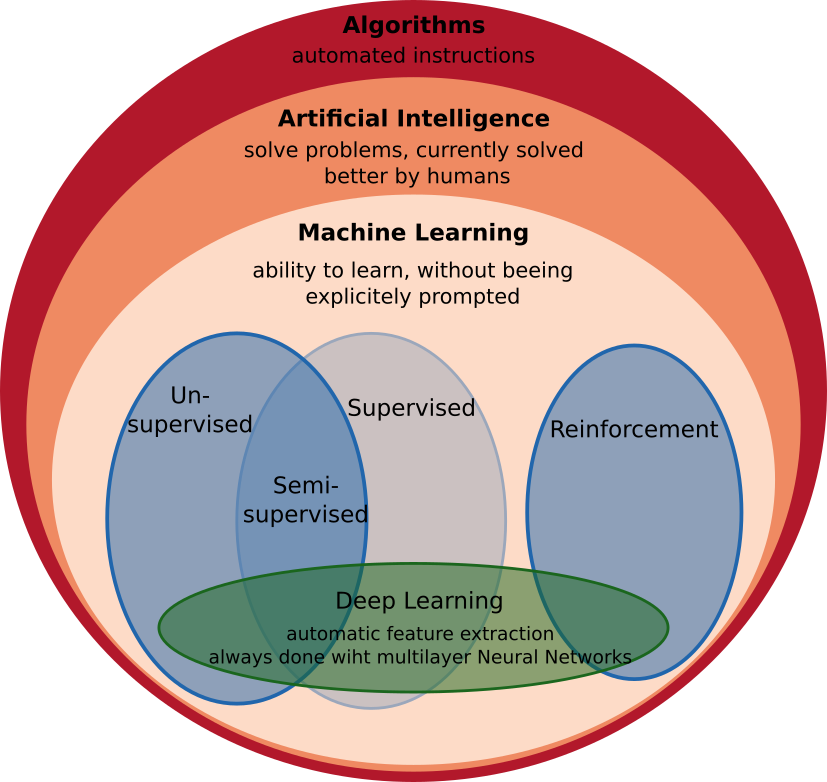
\includegraphics[width=0.85\textwidth]{pictures/contextML}\\
    \caption[Context of Deep Learning]{Visualisation of the context of Deep Learning in comparison to Algorithms, Artificial Intelligence, Machine Learning and the categories of learning algorithms. Machine Learning is a subset of Artificial Intelligence, which is a subset of all algorithms. Nested inside Machine Learning are the four categories Reinforcement Learning, Supervised and Unsupervised Learning as well as Semi-Supervised Learning(at the intersection of Supervised and Unsupervised Learning). Lastly, Deep Learning, which utilises multilayer do Neural Networks, is nested inside Machine Learning as well, but is not restricted to any category, rather spanning and exceeding all of them. Figure own work.}
    \label{fig:MLcontext}
\end{figure}

% ML categories
As shown before learning algorithms are classified depending on the nature of the feedback available to the system and Deep Learning algorithms are found in all of them.
Traditionally this means three categories: Supervised, Unsupervised, and Reinforcement Learning~\autocite{Burkov2019} (see \autoref{tab:MLtechniques}).
But in the last years another category was established: Semi-Super\-vised Learning, which combines Supervised and Unsupervised Learning to get the best of both categories~\autocite{Burkov2019}.

Image segmentation can be done with all of them, but usually the best results are today reached with Supervised Learning, though Unsupervised and Semi-supervised Learning are also found increasingly successful~\autocite[e.g.]{VanGansbeke2021}, as explained shortly.
Reinforcement Learning on the other hand, is better tailored to solve problems where the decision-making process is sequential (for example when playing video games or in navigation). %Reinforcement can be used for segmentation, but that is not classical application https://arxiv.org/abs/2002.06583
Thus, it will not be discussed in detail here.
\begin{table}[!htb]
    \caption[Learning techniques by category]{Overview of learning techniques by category, extracted from~\autocite{Sarker2021}. Completed with commonly used algorithms for traditional Machine Learning and Deep Learning from~\autocites{Mishra2020}{Moubayed2018}.}
    \label{tab:MLtechniques}
    \makegapedcells      % in makecell
    \begin{tabularx}{\textwidth}{|XXXX|}
        \hline
        \multicolumn{4}{|c|}{\textbf{\makecell{Machine Learning}}}            \\ \hline
        \multicolumn{1}{|c|}{\textbf{\makecell{Supervised\\Learning}}} & \multicolumn{1}{c|}{\textbf{\makecell{Unsupervised \\Learning}}} & \multicolumn{1}{c|}{\textbf{\makecell{Semi-\\Supervised \\Learning}}} & \multicolumn{1}{c|}{\textbf{\makecell{Reinforcement\\Learning}}} \\ \hline
        
        \multicolumn{1}{|>{\footnotesize}c|}{\makecell[l]{\textbullet~Classification \\ \textbullet~Regression}} &
        \multicolumn{1}{>{\footnotesize}c|}{\makecell[l]{\textbullet~Clustering\\ \textbullet~Association \\ \textbullet~Dimensionality \\~~~Reduction}} & \multicolumn{1}{>{\footnotesize}c|}{\makecell[l]{\textbullet~Classification\\ \textbullet~Clustering}} & \multicolumn{1}{>{\footnotesize}c|}{\makecell[l]{\textbullet~Classification\\ \textbullet~Control}} \\ \hline
        
        \multicolumn{1}{|>{\scriptsize}c|}{\makecell[tl]{Shallow algorithms:\\ \\\textbullet~Linear Regression\\ \textbullet~Logistic Regression\\ \textbullet~Support Vector\\~~~Machines\\ \textbullet~Decision Trees\\~\ldots}} &
        \multicolumn{1}{>{\scriptsize}c|}{\makecell[tl]{Shallow algorithms:\\ \\\textbullet~K-Means\\ \textbullet~Principal Component\\~~~Analysis\\~\ldots}} & 
        \multicolumn{1}{>{\scriptsize}c|}{\makecell[tl]{Shallow algorithms:\\ \\\textbullet~Self-Training\\ \textbullet~Low Density \\~~~Separation\\~\ldots}} &
        \multicolumn{1}{>{\scriptsize}c|}{\makecell[tl]{Shallow algorithms:\\ \\\textbullet~Q Net\\ \textbullet~Dynamic Programming \\ \textbullet~Monte Carlo Methods\\~\ldots}} \\ \hline
        
        \multicolumn{1}{|>{\scriptsize}c|}{\makecell[tl]{Deep algorithms:\\ \\\textbullet~Convolutional\\~~~Neural Networks\\ \textbullet~Recurrent Neural\\~~~Networks \\ \textbullet~Long Short Term\\~~~Memory\\ \textbullet~Transformers\\~\ldots}} &
        \multicolumn{1}{>{\scriptsize}c|}{\makecell[tl]{Deep algorithms:\\ \\\textbullet~Generative Adversary\\~~~Networks\\ \textbullet~Recurrent Neural\\~~~Networks \\\textbullet~Long Short Term\\~~~Memory\\ \textbullet~Transformers\\ ~\ldots}} & 
        \multicolumn{1}{>{\scriptsize}c|}{\makecell[tl]{Deep algorithms:\\ \\\textbullet~Autoencoders\\ \textbullet~Transformers\\ \textbullet~Restricted Boltz-\\~~~mann Machines\\ \textbullet~Deep Boltzmann\\~~~Machines\\~\ldots}} &
        \multicolumn{1}{>{\scriptsize}c|}{\makecell[tl]{Deep algorithms:\\ \\\textbullet~Deep Q Net\\ \textbullet~Deep Deterministic\\~~~Policy Gradients \\ \textbullet~Normalised Advantage\\~~~Functions\\~\ldots}} \\ \hline
    \end{tabularx}
\end{table}

%supervised learning: definition
Supervised Learning algorithms are trained on labelled data~\autocite{Burkov2019}.
This means for each training example a label is known, which represents the desired output of the model for this feature vector.
% application in medical segmentation
For image segmentation the training examples are numerical arrays representing pixel or voxel value, and the corresponding labels are again numerical arrays containing values indicating the assigned class for each voxel of the training example.
A lot of successful semantic segmentation algorithms use Convolutional Neural Networks, a supervised deep learning technique~\autocite{Antonelli2021}.

%disadvantages of Supervised algorithms and transition
The main drawback of supervised learning however, is the need for labelled data.
It is in the nature of labels that they must be assigned manually and often by experts, so data preparation takes a lot of time.

%unsupervised learning: definition
This is why today there are increasing efforts to leverage unsupervised learning techniques, which do not rely on labelled data, but can be used on unlabelled examples.
The aim of Unsupervised Learning algorithms is to find an arbitrary structure within the input without getting feedback from labels~\autocite{Burkov2019}\footnote{This means Unsupervised Learning is only suitable for certain tasks, like clustering, association rule learning, or dimension reducing, see~\autocite{Sarker2021}.}.
However, the patterns that Unsupervised Learning algorithms find might be connected to output prediction, but they do not necessarily need to be.
The meaning of the found patterns must ultimately be interpreted by a human~\autocite{Swana2021}.

%unsupervised learning: application on medical segmentation
Only recently an unsupervised deep learning algorithm for image segmentation on two-dimensional pictures has been presented~\autocite{VanGansbeke2021}.
But to date, no unsupervised algorithm is available for medical image data.
However, it can be expected, that these algorithms can be adapted to be used with medical data too, as will be shown in the following.
%However, it can be expected that more algorithms will be developed in the future, since computing resources are available and the need to finally skip the time-consuming labelling step for the training data prevails.

%Semi-Supervised: definition
Another approach in reducing the need of labelled data is Semi-Supervised Learning.
This is done by only providing some labelled training examples, which are then used to iteratively generate labels for the unlabelled examples~\autocite[Chapter 7.9]{Burkov2019}.
Thus, it lies right in between Supervised and Unsupervised Learning and was developed to solve regression and classification problems (as in Supervised Learning), but save on the time-consuming process of labelling all training examples (as in Unsupervised Learning)~\autocite{Burkov2019}.

% semi-supervised. application on medical segmentation
In medical image segmentation, Semi-supervised deep learning algorithms often improve results reached with pure supervised algorithms on the same data~\autocite{Chebli2018}.
However, to date the most successful algorithms for medical image segmentation still are supervised or semi-supervised algorithms~\autocite{Antonelli2021}, but it can be expected that more unsupervised algorithms will be developed in the future, since computing resources are available and the need to finally skip the time-consuming labelling step for the training data prevails.

\subsection{Deep Learning}\label{subsec:deep-learning}
%what Deep Learning can do
As previously illustrated, all successful algorithms used for medical image segmentation are Deep Learning algorithms, based on multilayer Neural Networks.
This is mainly due to the fact that they generally perform a lot better than traditional algorithms, especially when more data is available~\autocite{Mathew2021}.
Most traditional algorithms do not improve further once a certain data availability level is reached, while Deep Learning algorithms continue to enhance with more data~\autocite{Mathew2021}.

% advantage: no feature extraction
Another advantage is the increased independence from input quality and feature extraction in Deep Learning.
Usually, a lot of time and resources are used to manually clean up and prepare the data sets prior to training and features found in the raw data have to be transformed into suitable internal representations, so the algorithms understand them.

\begin{figure}[!htb]
    \centering
    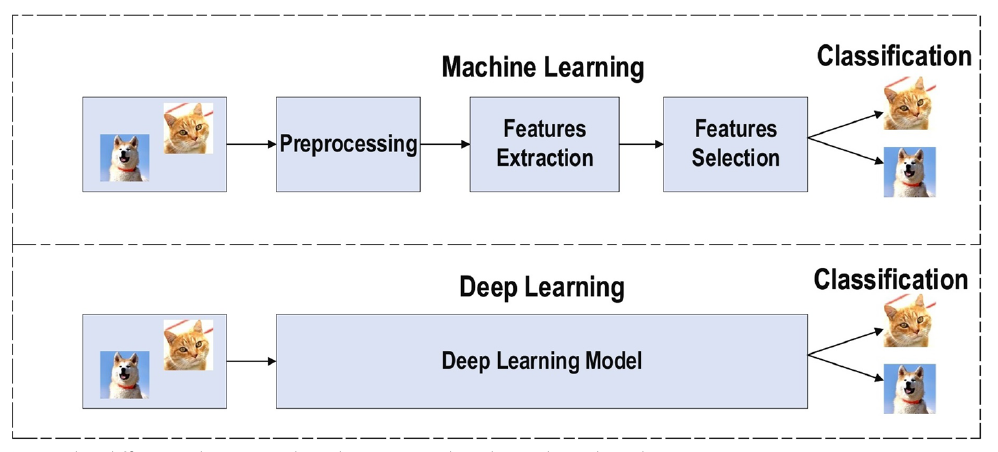
\includegraphics[width=\textwidth]{pictures/MLDLdiffrence}
    \caption[Work flow of learning algorithms]{Difference in the work flow of the algorithms in traditional Machine Learning and Deep Learning on the example of an classification tasks. In Deep Learning most preprocessing and feature extraction is done automatically, while in traditional Machine Learning human intervention is needed. Figure from ~\autocite{Alzubaidi2021}.}
    \label{fig:MLDLdiffrence}
\end{figure}
Each example is represented by a feature vector;
a vector containing values to describe the example in some capacity~\autocite{Burkov2019}.
For instance feature vectors in a data set describing flowers could contain a features to describe the colour as HEX value and another feature to describe the height in millimetre.
The position of the features in the vector is fixed, it must be the same throughout the data set.
So the first feature in the flower data set always needs to be the colour as HEX value, the second always the height in millimetre.
The process of generating these feature vectors from the raw data is called feature extraction.
In Deep Learning, multilayered Neural Networks are used, which means the model parameters are learned indirectly from the output of the previous layer~\autocite{LeCun2015}.
Thus, the feature extraction is automated and a lot less human intervention is needed (see \autoref{fig:MLDLdiffrence}).
In consequence, Deep Learning is very well scalable and can be used for huge data sets, which is crucial in most fields.

%Application of Deep Learning
Today Deep Learning is very successful in various domains, ranging from business, over governments, to science and medicine\autocite{LeCun2015}.
For some years now, Deep Learning algorithms regularly outperform other Machine Learning algorithms, for example at speech recognition~\autocite[e.g.][]{Hinton2012}, image recognition~\autocite[e.g.][]{Krizhevsky2010}, or natural language translation~\autocite[e.g.][]{Sutskever2014}\footnote{For a more comprehensive overview see~\autocite{LeCun2015}.}.
In medical image segmentation, Deep Learning algorithms even outperform human experts~\autocite{Antonelli2021}.

\subsection{Neural Networks}\label{subsec:neural-networks}
As mentioned before, all Deep Learning Algorithms rely on multilayer Neural Networks.
% very short history
Originally, Neural Networks relied on the idea to model biological neurons and especially the connection of neurons (since the connections carry the real information), to enable computers to learn in the same way humans do~\autocite{Ertel2017}.
This idea dates back to 1957, when \citeauthor{Rosenblatt1957} introduced the perceptron, a device used to classify images ~\autocite{Rosenblatt1957}.
But only in the 1980s, when the backpropagation algorithm was developed multilayer networks became possible~\autocite[Chapter~1.3]{Skansi2018} and the scope of application for Neural Networks became much broader.
In 2006~\citeauthor{Hinton2006} coined the term Deep Learning for multilayer Neural Networks and proposed a new training strategy~\autocite{Hinton2006}.
An explosion of papers on different network architectures followed, which aimed at solving a multitude of problems, ranging from natural language translation, to cyber-security, or medical image segmentation~\autocite[Chapter~1.3]{Skansi2018}.
One of these architectures, the Vision Transformer, will be explained in detail later (see~\autoref{subsubsec:visiontransformer}).

%short explanaition of neuron
All of these architectures however, are based on Artificial Neural Networks which consist of neurons.
Each neuron is appointed a set of weights which are multiplied with the input(s) to calculate the output of that neuron (see \autoref{fig:neuron}).
Learning is done by purposefully adjusting the weights, so the output of the neural network will be closer to the desired output.
The major problem of multilayer networks has been the inability to decide how much the individual weights of each neuron have to be changed.
But backpropagation solved this problem by simply utilising the derivative of the loss function~\autocite{Rumelhart1988}, as explained in~\autoref{subsubsec:backward-pass}.

%A more comprehensive timeline on the history of Artificial Intelligence and Machine Learning can be found in~\autocite{Mathew2021} and in~\autocite[Chapter~1.2.2]{Ertel2017}.

\subsection{Structure of an artificial Neuron}\label{subsec:structure-neuron}
%Neurons today, pretty much rely on the same principles as the perceptron introduced by~\citeauthor{Rosenblatt1957} in 1957. In case i need to explain the perceptron: \autocites[Chapter~4.3]{Skansi2018}[Chapter~1.2.1]{Aggerwal2018}
As explained briefly before, artificial neurons are appointed a set of weights $w$, which are multiplied with the inputs $x$ and summed up to calculate the output $y$ of that neuron (see \autoref{fig:neuron}).
After summation, a function $f$ is applied to map the outputs to a defined number space.
\begin{equation}
    y = f(\sum^n_{i=1}w_ix_i)
    \label{eq:single-neuron}
\end{equation}
Or, expressed as a vector calculation, with $\vec{w}$ being a $1 \times n$ vector and $\vec{x}$ a $n \times 1$:
\begin{equation}
    y = f(\vec{x}w^T \vec{x})
    \label{eq:single-neuron-vector}
\end{equation}

\begin{figure}[!htb]
    \centering
    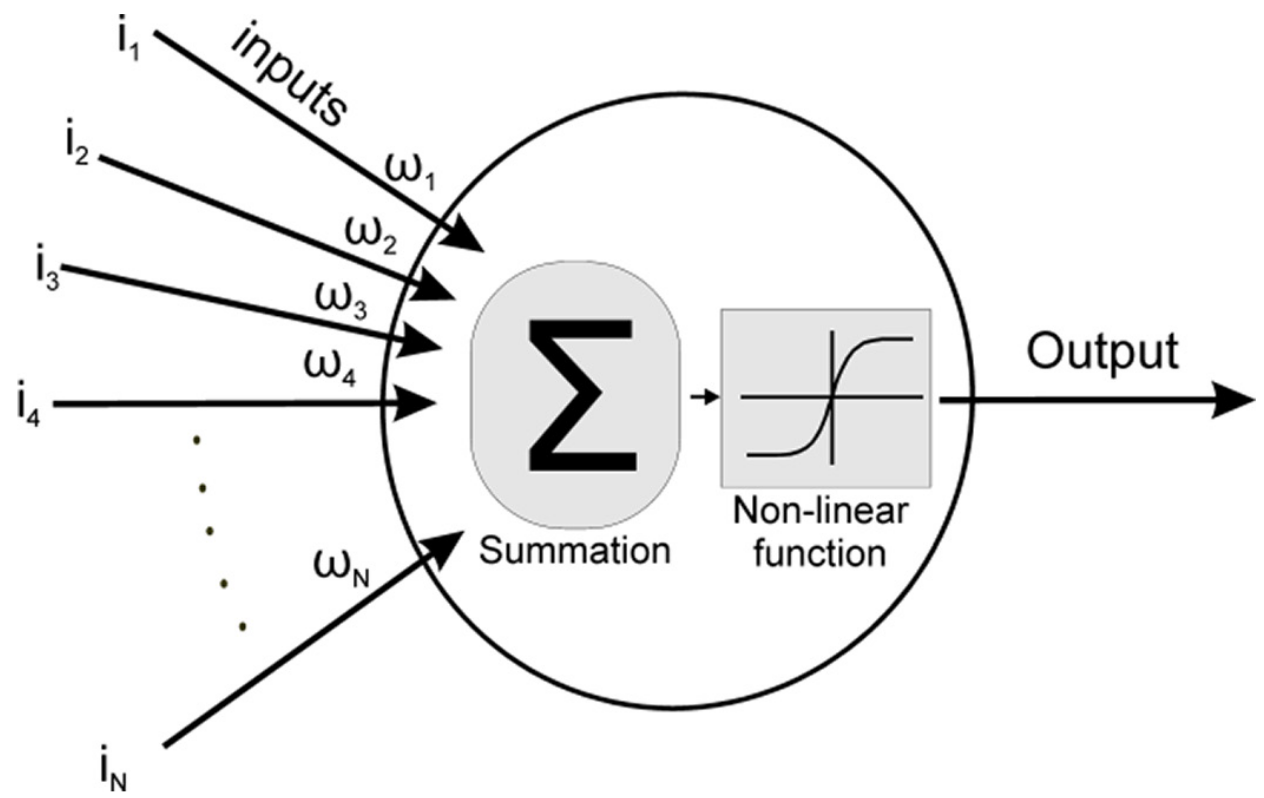
\includegraphics[width=0.7\textwidth]{pictures/neuron}
    \caption[Schema of an artificial neuron]{Schematic diagram of an artificial neuron. From left to right: inputs ($i_1$–$i_n$) are multiplied with synaptic weights ($\omega_1$–$\omega_n$), the products are added ($\sum$), and the result is passed to a nonlinear function to produce the output. Figure from~\autocite{Pouliakis2016}.}
    \label{fig:neuron}
\end{figure}

%Activation function
The function which is applied after summation to map the output to a defined number space is called activation function.
The choice of the activation function is dependent on the number space of the desired output.
For example, a sigmoid function can be applied to generate a binary classifier (output can be either zero or one), a \gls{relu} function is used for prediction of positive integers, and Softmax for probabilistic values (since the range of the function is between zero and one)~\autocite{Sharma2020}, see \autoref{fig:activation-functions}.\footnote{By choosing a suiting activation function, most shallow deep learning techniques can be simulated with a single-layer network~\autocite[Chapter~1.2.1]{Aggarwal2018}.}
Today many activation functions are available, each adapted to different problem domains and network architectures, as seen in \autoref{fig:activation-functions} (for a more comprehensive overview see~\autocite{Sharma2020}).
%In multilayer networks activation functions needs to be non-linear, so the backpropagation algorithm can work, as explained below.
\begin{figure}[!htb]
    \centering
    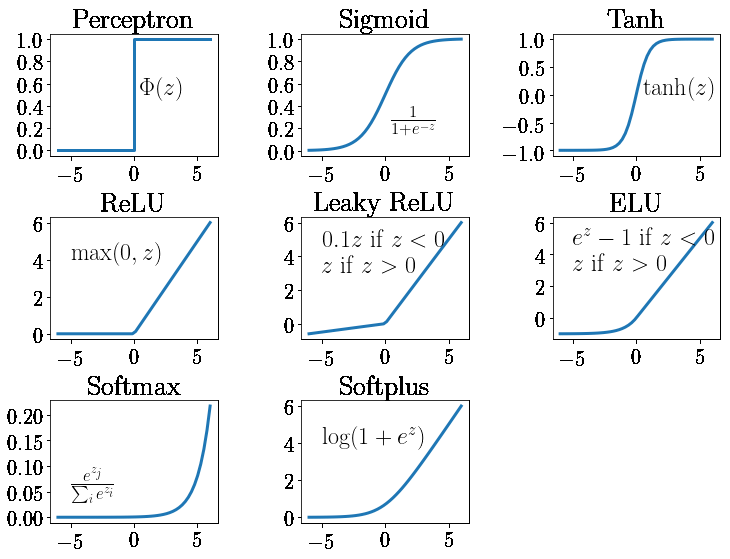
\includegraphics[width=\textwidth]{pictures/activation_functions}
    \caption[Common activation functions]{Common activation functions in Artificial Neural Networks, to introduce non-linearity. The sigmoid is the archetype activation function because the closed form solution for the derivative of the sigmoid, which is used during model fitting, is an excellent pedagogical tool; however, the rectified linear unit is, at present, the most common activation function in the hidden layers. Figure and caption from~\autocite{Johnson2020}.}
    \label{fig:activation-functions}
\end{figure}

%bias
When adding a constant input to a neuron (called a bias $b$), single neurons can be used as linear classifiers, with the bias representing the y-intercept in two-dimensional spaces~\autocite{Ertel2017} (see \autoref{fig:linear-separable}).
\begin{equation}
    y = f(b + \sum^n_{i=1}w_ix_i)
    \label{eq:single-neuron-bias}
\end{equation}
Or, expressed as a vector calculation, with $\vec{w}$ being a $1 \times n$ vector and $\vec{x}$ a $n \times 1$:
\begin{equation}
    y = f(b + \vec{x}w^T \vec{x})
    \label{eq:single-neuron-vector-bias}
\end{equation}


%learning/training
Learning or training is done by iteratively adjusting the weights of the neurons.
The training phase is commonly referred to as backwards pass, while the calculation of the output is called forward pass.


\begin{figure}[!htb]
    \centering
    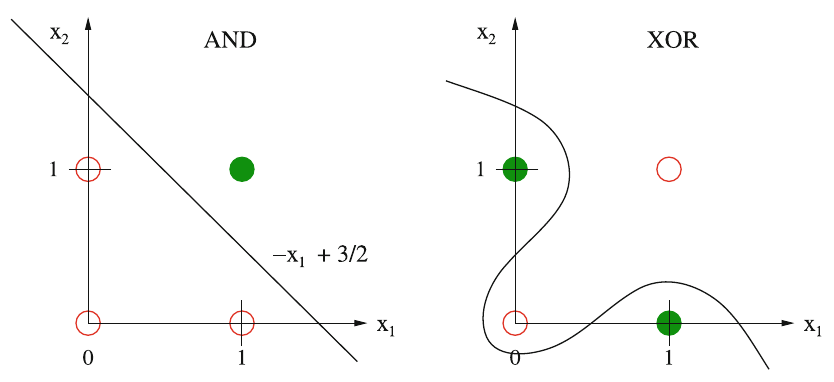
\includegraphics[width=0.8\textwidth]{pictures/linear-separable}
    \caption[Linear separable and inseparable data sets]{Linear separable and inseparable data sets. On the left side a representation of the AND function is seen, on the right side a representation of XOR. Filled green dots represent true, red framed dots false. 
    For the AND function a linear separator can be drawn through the coordinate system to separate true from false. For XOR, this is only possible with a non-linear separator. Figure from~\autocite{Ertel2017}.}
    \label{fig:linear-separable}
\end{figure}

\subsection{Multilayer Networks}
Some problems can only be solved by multilayer networks (e.g.~non-linear classifiers as used in image segmentation).
Multilayer networks are created by using the output of one layer of neurons as input for the next layer (see \autoref{fig:MLP}).
Usually, there are no interlayer connections and all neurons of the previous layer are connected to all neurons of the next layer, but this may change with the network architecture~\autocite[Chapter~1.2.2]{Aggarwal2018}.
\begin{figure}[!htb]
    \centering
    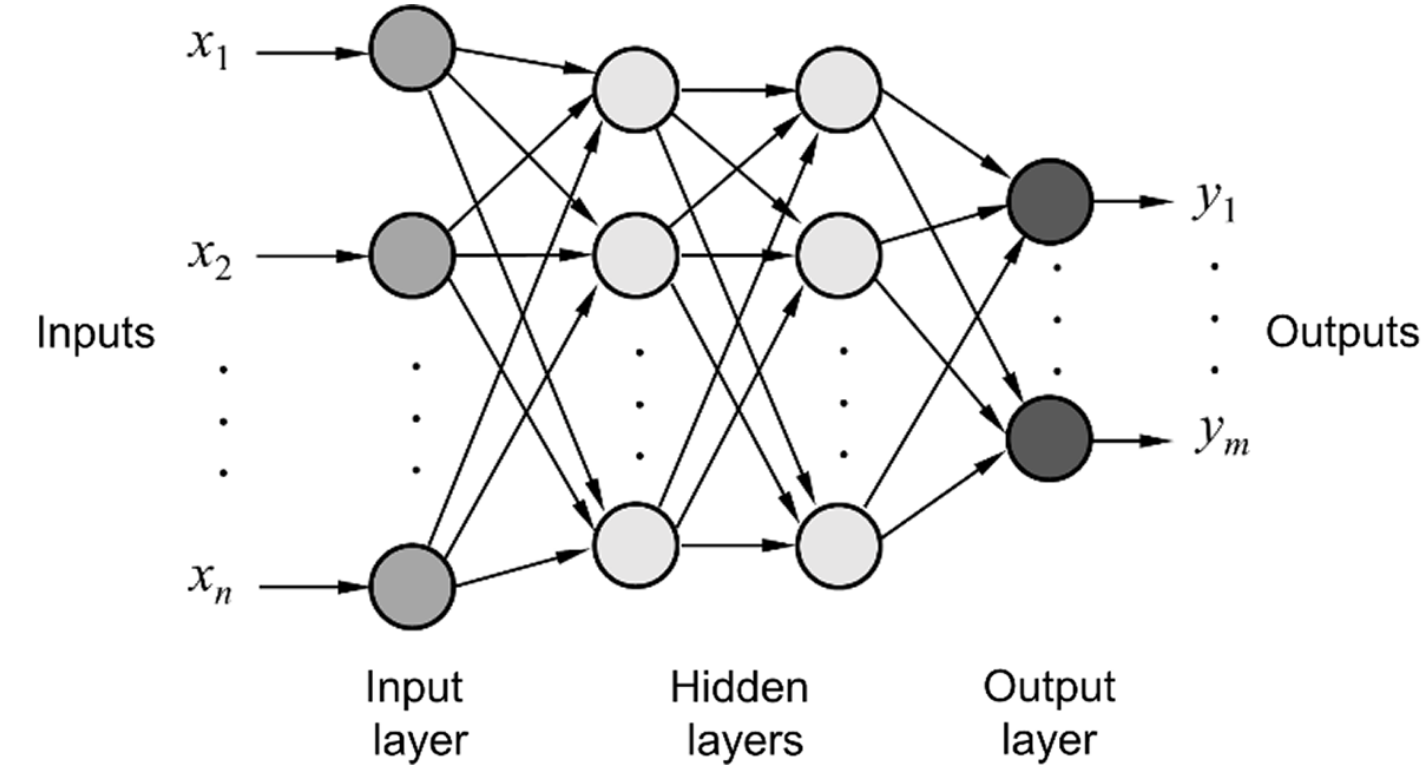
\includegraphics[width=0.9\textwidth]{pictures/MLP}
    \caption[Typical structure of multilayer neural networks]{Typical structure of a multilayer neural network. Every neuron of a layer is connected to all neurons of the following layer. No connections within a layer are present. Figure from~\autocite{Pouliakis2016}.}
    \label{fig:MLP}
\end{figure}

%inputs
For each feature of the input vectors, one neuron in the input layer is generated.
%hidden layers
The layers between input and output are called hidden layers, because the performed computations are not visible to the user~\autocite[Chapter~1.2.2]{Aggarwal2018}.
The number and configuration of hidden layers is specific for each architecture.
%outputs
The number of neurons in the output layer depends on the desired output and the activation function of this layer~\autocite[Chapter~1.2.1]{Aggarwal2018}.
For example, if a classification problem is solved, a Softmax function with one output neuron for each class can be used to generate a probabilistic output value for each class.
In an Autoencoder however, the number of output neurons will be the same as the number of input neurons, since the (unsupervised) network will try to reproduce the input~\autocite{Aggarwal2018}.
Note that the layers do not need to use the same activation functions, but usually the activation function within a layer are the same~\autocite[Chapter~1.2]{Aggarwal2018}.
%activation functions
Especially the output layer utilises different activation functions depending on the intended output number space (as explained before), while hidden layers mostly use \gls{relu}~\autocite{Johnson2020}.


\subsubsection{Forward Pass}
%forward pass
The output of a multilayer network can be represented by a simple matrix calculation as seen in \autoref{fig:forwardpass-layer}.
In each neuron the activation function $f(.)$ is applied to the sum of the weighted inputs.
This output of a neuron is then used as input for the next layer, where again the activation function is applied on the sum of weighted inputs.
This is repeated until the output layer is reached.

\begin{figure}[htb]
    \centering
    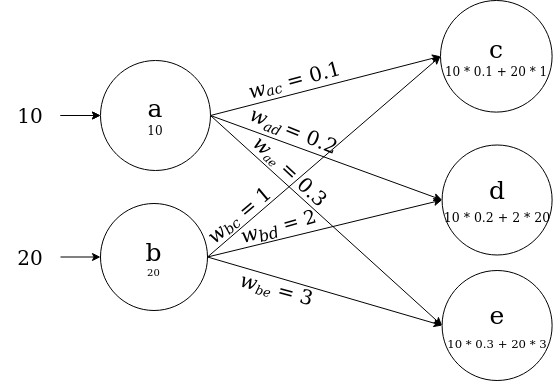
\includegraphics[width=0.75\textwidth]{pictures/forwardpass_1layer}
    \caption[Forward pass through neural network]{
    Forward pass through one layer of a neural network. Each output is a weighted input for the next neuron. In each neuron the weighted inputs are summed. For simplicity activation functions have been omitted. Figure adapted from~\autocite[Chapter~4.2]{Skansi2018}.}
    \label{fig:forwardpass-layer}
\end{figure}

The weights connecting two layers can be represented as a matrix, for example, for the weights given in \autoref{fig:forwardpass-layer} the matrix is~\autocite[Chapter~4.2]{Skansi2018}:
\begin{equation}
    \begin{bmatrix} 
	    w_{ac} & w_{ad}  & w_{ae}  \\
	    w_{bc}  & w_{bd}  & w_{be} \\
	\end{bmatrix}
    =
	\begin{bmatrix} 
	    0.1 & 0.2 & 0.3  \\
	    1  & 2  & 3 \\
	\end{bmatrix}
    \label{eq:forward-matrix}
\end{equation}
Thus, the weighted sum of inputs $z$ to a neuron can be represented as a matrix calculation of the weight matrix $U$ of the previous layer and the input vector $\vec{x}$ of that layer:
\begin{equation}
    z = \sum U *\vec{x}
    \label{eq:forward-matrix-calc}
\end{equation}
At each layer $l$ of a network function $n_l$ is calculated.
Thus, the connection of the layers to each other is a nested application of these functions, for example the layers $input$, $hidden$, and $output$ with the input vector $\vec{x}$ connect to each other like this: $n_{output}(n_{hidden}(n_{input}(\vec{x})))$~\autocite[Chapter~4.3]{Skansi2018}.

\subsubsection{Backward Pass}\label{subsubsec:backward-pass}
%backward pass
So, the forward pass in a multilayer network is relatively easy.
However, training the network, also referred to as backwards pass, is more complex, since it must be decided how much an individual weight needs be adjusted, according to how much it contributes to the result of the network.
In multilayer networks, this weight adjustment is cast to a search or optimisation problem, mostly optimising the loss function.

\paragraph{Loss Function} \label{subsubsec:lossfunction}
The loss function is the central point of any Neural Network: It quantifies the difference between the expected and the actual output of a network and is the function that is optimised during training.
The loss function thus highly depends on the problem statement~\autocite[Chapter~1.2.1]{Aggarwal2018}.

In supervised learning the loss function quantifies the difference between network output and ground truth.
For example for multicategorical output (as found in image classification) often the cross entropy-loss (\autoref{eq:entropy-loss}) is used, where $\hat{y}_i$ is the probability of the classes and the $r$-th class is the ground truth~\autocite[Chapter~1.2.1]{Aggarwal2018}.
Note that, if the number of classes in this model is two, it will perform a logistic regression, so this is a generalisation of logistic regression.
\begin{equation}
    E = -\log(\hat{y}_r)
    \label{eq:entropy-loss}
\end{equation}
For supervised image segmentation often the more specialised dice loss is utilised, which relies on the \gls{dsc}, as explained in \autoref{subsubsec:model-performance-assessment}~\autocite{Jadon2020}:
\begin{equation}
    E = 1 - \frac{2y\hat{p}+ 1}{y + \hat{p} + 1}
    \label{eq:dice-loss}
\end{equation}
In this context $\hat{p}$ denotes the Softmax output of the network.
To ensure that the function is not undefined in edge cases, 1 is added to nominator and denominator.

With unsupervised learning however, the ground truth is not available\footnote{This is also the reason, why only some tasks can be solved with unsupervised learning.}, thus another optimisation criterion need to be utilised.
Generative Advisory networks, which are used to produce further examples matching the input distribution, consist of two networks, a Generator and a Discriminator, which try to out-compete each other~\autocite{Goodfellow2020}.
%Contrastive loss for unsupervised
Other approaches comprise contrastive techniques, where an instance discrimination task is done, for example by differentiating positive view pairs (crops or distortions from same or similar images) with negative view pairs (from different images)~\autocite{Wang2021}, as will be explained exemplary in~\autoref{subsec:stego-loss-function}.

\paragraph{Backpropagation}
The remaining question for weight adjustment is: How exactly is the loss function optimised in the backwards pass?
As mentioned earlier, this is done through a gradient descent method called backpropagation.
Backpropagation utilises the chain rule to calculate the derivative (the gradient) of the loss function with respect to the specific weight~\autocite[e.g.][]{Aggarwal2018}.
This gradient can then be used to adjust the weight $w_i$ in question by subtracting a fraction ($\eta$) of the gradient from the weight (\autoref{eq:weight-update-single}) and (\autoref{eq:weight-update-vector})\footnote{The relevance of $\eta$ is explained in further detail at the end of this section.}.
\begin{equation}
    w^{new}_i = w^{old} -\eta \frac{\partial E}{\partial w^{old}}
    \label{eq:weight-update-single}
\end{equation}
This can also be noted in vector notation for all weights of a neuron ($\vec{w}$ denotes a vector of weights of a neuron and $E$ a matrix of partial derivatives with respect to the single weights):
\begin{equation}
    \vec{w}^{new} = \vec{w}^{old} -\eta \nabla E
    \label{eq:weight-update-vector}
\end{equation}
%Nabla operator: Vector of all partial derivatives (or matrix if multiple functions)
For a more detailed explanation on how to calculate the gradient see~\autocite{Ruder2017}.

By working backwards from the output layer, the weight adjustment propagates through all layers, thus the name of the algorithm.
Note that both the activation function, and the loss function need to be non-linear, as they have to be differentiable for backpropagation to work~\autocite{Aggarwal2018}.

% epochs
Weight adjustment is done throughout the whole network, multiple times for all training examples.
One run through all training examples is called an epoch and a network is trained for several (often hundreds or thousands of) epochs~\autocite[Chapter~4.7]{Skansi2018}.
However, in some architectures epochs can be defined by a fixed number of examples (e.g.~\autocite{Isensee2021}).

% stochastic/mini/batch gradient descent
There are different approaches to gradient descent methods, differentiated by the amount of training examples used to calculate the gradient of the loss function.
This can generally be seen as a trade-off between accuracy and calculation time~\autocite{Ruder2017}.
When the gradient is calculated separately for each training example, the method is called Stochastic Gradient Descent.
Weights are adjusted often and with high variance, which leads to a heavily fluctuating loss function~\autocite{Ruder2017}.
On the other hand, it can be used online (while adding new examples to the training set) and is fast~\autocite{Ruder2017}.
In Batch Gradient Descent the network parameters are updated only after all training examples are considered, by calculating the gradient of the whole network.
This takes a lot of memory and time, and it can only be used for small data sets, which fit completely into memory~\autocite{Ruder2017}.
To combine the best of both worlds, Mini-batch Gradient Descent was developed, where the gradient is calculated for a group of training examples (depending on the application and available memory 50 to 256 examples)~\autocite{Ruder2017}.
It has a stable convergence and is relatively fast and memory efficient.
Thus, this approach is deployed in most modern Neural Networks~\autocite{Ruder2017}.
%modified gradient descent
To further accelerate the learning process, methods are often adjusted further by use of e.g.~the Adaptive Gradient Algorithm, Root Mean Square Propagation, Adam optimiser, or gradient descent with Nesterov momentum (for details see~\autocite[Chapter~3.5.1]{Aggarwal2018}).

% learningrate policy
As explained before, the weights of the network are adjusted during training.
However, adjustment will only be done by a small fraction $\eta$, the learning rate.
This way weights will only change considerably, when a lot of training examples support that direction.
This generally avoids overfitting, where the model performs well on the training data but poorly on unknown test data.\footnote{Overfitting can be compared to a human having learned the examples by heart and not generalising to a broader context~\autocite{Alzubaidi2021}.}
There are several other more refined techniques to avoid overfitting, as explained in~\autocite[Chapter~5.3]{Skansi2018}, but it all starts with the learning rate.

% learning rate decay
Usually, the learning rate is not fixed, but will decay over time~\autocite[Chapter~3.5.1]{Aggarwal2018}.
This way, at the beginning of the training, when weights are probably further away from their optimum, they are adjusted more (making the whole training process faster) and later, when they are already closer to their optimum, they will be adjusted less, to prevent oscillation around the optimum or even missing the optimum entirely~\autocite[Chapter~3.5.1]{Aggarwal2018}.

%For image segmentation, a polynomial learning rate seems to be most efficient, where adjustment is done by multiplying the base rate with a polynomial factor dependent on the iterations~\autocite{Mishra2019}:
%\begin{equation}
%    \eta_t = \eta_0 * (1 - \frac{i}{T_i}^p)
%    \label{eq:polynomial-decay}
%\end{equation}
%With $\eta_0$ as initial learning rate, $p$ as fixed value between 0 and 1 to control the shape of the polynomial curve, $i$ is the iteration and $T_i$ the overall number of iterations.


\subsubsection{Model Performance Assessment} \label{subsubsec:model-performance-assessment}
Once the training of a network is finished, and all weights are set to somewhat optimal values, the network represents a model, which can be used to predict results for unknown input.
To assess model performance, it is used on a data set not used during training (the validation or test set) and predictions are compared to the ground truth.

For classification tasks, the most frequently used assessment metrics rely on the confusion matrix~\autocite{Reinke2022}.
It has two axis, comprising the predicted and actual labels, as seen in \autoref{tab:confusion-matrix}.
In a binary classification task four cardinalities are defined, but it can be easily extended for multilevel classifications by adding a row and column for each label~\autocite{Reinke2022}.
Cardinalities are:
\begin{itemize}
    \item true positives: examples that are correctly predicted to belong to a specific label
    \item false positives: examples that are incorrectly predicted to belong to a specific label
    \item true negatives: examples that are correctly predicted as not belonging to a specific label
    \item false negatives: examples that are incorrectly predicted to not belong to a specific label
\end{itemize}

\begin{table}[!htb]
    \centering
    \caption[Confusion matrix]{Confusion matrix for a binary classification task with the labels \emph{yes} and \emph{no}. It characterises the capabilities of a model by comparing the numbers of actual and predicted examples for each label. The sum within a row gives the number of actual examples with that label, the sum of a column the number of actually predicted examples of that label. The four cardinalities of the table (True Positive, False Positive, True Negative, False Negative) are used to calculate metrics that indicate model performance.}
    \label{tab:confusion-matrix}
    \makegapedcells
    \begin{tabular}{cc|c|c}
        \multicolumn{2}{c|}{}  &   \multicolumn{2}{c}{\textbf{Predicted}}  \\
        &             &      yes       &      no         \\
        \cline{1-4}
        \multirow{2}{*}{\rotatebox[origin=c]{90}{\textbf{Actual}}}
        & yes         & \makecell{True Positive \\ (TP)}  &  \makecell{False Negative \\ (FN)} \\
        \cline{2-4}
        & no          &  \makecell{False Positive \\ (FP)} &  \makecell{True Negative \\ (TN)}   \\

    \end{tabular}
\end{table}

The values of the confusion matrix can be used to calculate different metrics, for example Precision, Recall and Accuracy (see~\autocite{Reinke2022} for more details).

%semantic image segmentation assessment score:
Two of the most commonly used metrics for in computer vision and medical image segmentation tasks are the \gls{dsc} and \gls{iou}~\autocite{Reinke2022}.
%DSC
The \gls{dsc} (or F1-score) indicates the overall overlap between the predicted and the actual labels of all pixels (or voxels) as value from 0 (no overlap) to 1 (full overlap)~\autocite{Reinke2022}.
For a single label it is defined as:
\begin{equation} 
    DSC = \frac{2TP}{2TP + FP + FN}
    \label{eq:dsc}
\end{equation}
%IoU
The \gls{iou} (or Jaquard-index) is defined as the ratio of area of overlap and area of union, hence the name~\autocite{Reinke2022}.
tp / (tp + fp + fn)
\begin{equation}
    IoU = \frac{TP}{TP + FP + FN} \text{ or } IoU_{A,B} = \frac{|A \cap B|}{|A \cup B|}
    \label{eq:IoU}
\end{equation}
\gls{iou} and \gls{dsc} are related, as the \gls{dsc} of two sets$A$ and $B$ can also be expressed via the \gls{iou} of these sets~\autocite{Reinke2022}:
\begin{equation}
    DSC_{A,B} = \frac{2IoU_{A,B}}{1 + IoU_{A,B}}
    \label{eq:dsc-IoU}
\end{equation}
When evaluating these metrics, it has to be taken into account, however, that it is just an average and it may be especially misleading when small areas are compared, where a difference of one pixel has high impact~\autocite{Reinke2022}.
Moreover, it has to be kept in mind that even domain experts often disagree on the exact boundaries of objects in an image and so minor displacements of borders maybe should be penalised lesser, than full areas that do not match.
This has to be taken into consideration at model evaluation, and it is always a good idea to not rely solely on the metric, but also have a look on the predictions made.
%NSD
%This is where distance-based metrics like \gls{nsd} come into play.
%\gls{nsd} also measures overlap between two areas $A$ and $B$, but it tolerates some difference between them by defining boundaries $S$ and border regions $\mathcal{B}$ of width $\tau$~\autocite{Reinke2022} (see \autoref{fig:nsd}):
%\begin{equation}
%    NSD_{A,B}^{(\tau)} = \frac{|S_A \cap \mathcal{B}_B^{(\tau)}| + |S_B \cap \mathcal{B}_A^{(\tau|)}}{|S_A| + |S_B|}
%    \label{eq:nsd}
%\end{equation}

%\begin{figure}[!htb]
%    \centering
%    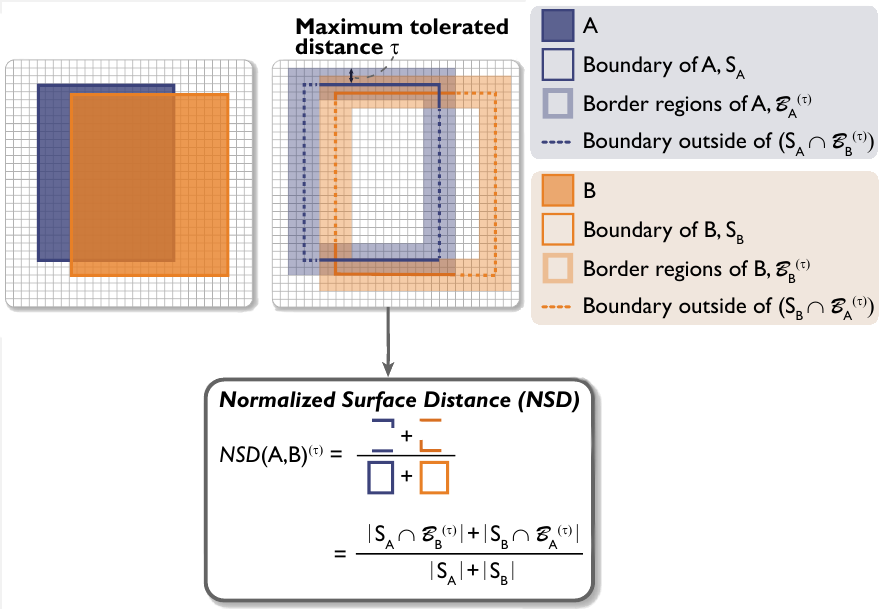
\includegraphics[width=\textwidth]{pictures/nsd}\\
%    \caption[Visualisation of Normalised Surface Distance]{Visualisation of calculation of \gls{nsd}. Calculates the overlap between two areas $A$ and $B$, but allows for some displacement between areas, by defining a border region $\mathcal{B}$ of width $\tau$. Figure from~\autocite{Reinke2022}}
%    \label{fig:nsd}
%\end{figure}

% limitations of metrics
%When selecting a metric to evaluate a model, the different advantages and limitations must be considered with respect to the task at hand, as explained by~\autocite{Reinke2022}.

% cross validation
Other ways, to improve model performance are resampling methods.
In the most basic set-up available data will be split into train and test set.
The model will be trained on the training set and validation metrics will be calculated on the test set to estimate model performance (the models generalisation capacities).
This leaves out a considerable amount of data from the training, and might bias the resulting model.
To mitigate this, often resampling methods are used, where multiple models are trained on different train test splits~\autocite[Chapter 5]{James2013}.
The averaged performance of these models, estimates the performance of the final model (trained on the full data set)~\autocite[Chapter 5]{James2013}.
 Usually in Machine Learning, k-fold cross validation is done, where the data is split into k sets (or folds) and every fold is used as validation set exactly once~\autocite[Chapter 5]{James2013}.
In practice, k is often set to 5 or 10, depending on the amount of data available~\autocite[Chapter 5]{James2013}.

A special case of cross-validation is leave-one-out cross-validation, where the data set is split into $n$ folds ($n$ indicating number of samples in the data set).
So, $n$ models are trained, and during each training exactly one sample is used as validation set~\autocite[Chapter 5]{James2013}.
Especially with smaller data sets a leave-one-out tactic is often recommended, since it is trained on a more representative training set, thus reducing the bias of the model~\autocite[Chapter 5]{James2013}. %https://codesachin.wordpress.com/2015/08/30/cross-validation-and-the-bias-variance-tradeoff-for-dummies/
However, using only one sample as validations set might lead to a higher variance during evaluations, since inhomogeneities and outliers in the data will have more influence when used alone for validation~\autocite[Chapter 5]{James2013}.
On the other hand, it was found out by \citeauthor{Bengio2004}, that high correlation of training sets may also lead to a higher variance in leave-one-out cross-validation~\autocite{Bengio2004}. %https://stats.stackexchange.com/questions/61783/bias-and-variance-in-leave-one-out-vs-k-fold-cross-validation
So performance on leave-one-out cross-validation might vary between data sets.

\subsection{Transformers} \label{subsec:transformer}
% http://nlp.seas.harvard.edu/2018/04/01/attention.html#position-wise-feed-forward-networks
% Transformer - Overview
Originally, Transformers were developed for (supervised) language processing tasks, Transformers accept sequential input data (e.g.~words in a sentence), while allowing parallel processing~\autocite{Vaswani2017}.
This sets them apart from the former state-of-the-art in natural language processing (like e.g.~Recurrent or Convolutional Neural Networks).
In contrast to most other Networks, Transformers are solely based on an attention mechanism, which can easily be parallelised and require less computational power, which means they often reach better results with less recources~\autocite{Vaswani2017}.
%They were originally designed for language processing tasks, like machine translation or next sentence prediction, but where soon adapted to computer vision tasks like image classification, object detection or image segmentation and today there is a vast number of architectures adapted for different tasks available~\autocite{Lin2021}.
Like all Encoder-Decoders Transformers map an input token to an output token via an intermediate representation of inputs, in which hopefully all relevant features are encoded.
For natural language processing this usually means mapping input words to output words.

% Transformers for images
However, they were soon adapted to be applied to image classification,, and are now even successfully used for image segmentation tasks~\autocite{Liu2019}.
%Since Transformers allow for significantly more parallelisation, reached better results with less resources in language processing tasks, and can today be even used in unsupervised settings, they were soon adapted to be applied to images, and are today successfully used for image segmentation~\autocite{Liu2019}.
In contrast to most state-of-the-art image segmentation methods, Vision Transformers have the potential to be trained fully unsupervised~\autocite{Hamilton2022}, making it very relevant for scientific application, where often no labeled data is available.
However, Vision Transformers were found to require more data in comparison, as discussed in~\autocite{Coccomini2021}.

\subsubsection{Model Structure}
% Transformer - Model Structure
% https://www.wikiwand.com/en/Transformer_(machine_learning_model)#Architecture
As seen in \autoref{fig:transformer}, Transformers implement an Encoder-Decoder model structure, without using convolutions or recurrence, and instead replacing it with multi-head attention and point-wise feed forward networks.
\afterpage{
    \begin{figure}[!t]
        \centering
        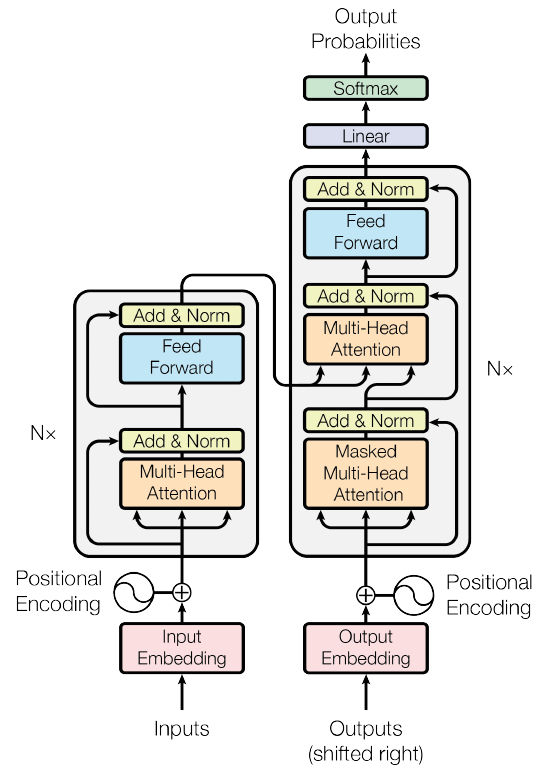
\includegraphics[width=0.75\textwidth]{pictures/transformer}\\
        \caption[Transformer model Structure]{Transformer model Structure. The transformer consists of a encoder (left side) and a decoder (right side). The encoder comprises a multi-head self-attention sub-layer and a fully connected feed forward sub-layer. Each sublayer has residual connections to the respective input, which is added to the output and normalised.\\The decoder is structured similarly, but has an additional intermediate layer, where cross-attention with the encoder output is calculated. Also the self-attention sub-layer in the decoder is masked, to prevent positions from attending to subsequent positions. The last step in the decoder is a linearisation and softmax application, so the output will be probabilities per token.\\ Inputs and Outputs are embedded via a learned function (with shared weights) get a positional encoding (based on sind and cosine functions). In the decoder the output embedding is shifted right, again to ensure that predictions only depend on former positions. Figure from~\autocite{Vaswani2017}}
        \label{fig:transformer}
    \end{figure}
    \clearpage
}

% Encoder
The encoder consists of a stack of six layers, each of which contains a multi-head self-attention mechanism and a simple positional-wise fully connected feed-forward network.
%The feed forward network consists of two linear transformations with a \gls{relu} function, which is similar to two convolutions with kernel size one~\autocite{Vaswani2017}.
The attentions, are passed to this network, to transform them to a rich representation~\autocite{Vaswani2017}.
This will adjust for bad initialisation parameters and also hinders rank collapse. %https://theaisummer.com/transformer/
\citeauthor{Geva2021} even found, that the feed forward layer actually acts as key value store~\autocite{Geva2021}(for an explanation of keys and values see~\autoref{subsubsec:attention-mechanism}).
A residual connection of the previous sub-layer is added to the result of each sub-layer before normalisation is applied.
The residual connections and normalisation help mitigate the vanishing gradient problem~\autocite{Wang2019}. %, and also ensure that the contextual representations of the (original)input tokens actually represent the tokens https://stats.stackexchange.com/questions/565196/why-are-residual-connections-needed-in-transformer-architectures

% Decoder
Like the encoder the decoder also consists of a stack of six layers, but additionally has a middle sub-layer, where multi-head-attention over the output of the encoder stack is done.
Additionally, the multi-head attention sub-layer is modified to prevent positions from attending to subsequent positions by masking the corresponding inputs.
This, and shifting the output embedding by one position, ensures that predictions for a token can only depend on the positions before that token.
The decoder output is converted to predictions (next token probability) by applying a learned linear transformation with a softmax function.~\autocite{Vaswani2017}

% Token embedding
The input and output tokens are embedded\footnote{Embedding: "translating" higher dimensional tokens to lower dimensional spaces. E.g. converting a token to a vector} using a learned function~\autocite{Vaswani2017}.
The embedding layers share their weights with the linear pre-softmax layer of the output, since it was found that this enhances embedding quality~\autocite{Press2017}.
%positional encoding (this was formerly done with convolution / revurrence)
Additionally, the resulting vectors will be encoded positionally.
Since skipping convolution and recurrence completely, means that the position of tokens needs to be coded explicitly, so the order of the sequence can be used by the algorithm.
This is done by mapping the positions to a sinusoid function, as it is theorised, that this will help the model learn relative positions and adding them to the embedded token.~\autocite{Vaswani2017}

%? training and loss function
Training is done via backpropagation and the weights adjusted are: the weights for the embedding layers, the feed-forward layer weights and the weight matrices to calculate Q, K, V (as explained in~\autoref{subsubsec:attention-mechanism}) in encoder and decoder and the weights fo the final linear layer.
The optimised loss function is the cross-entropy loss, which is often used for probability distributions in supervised learning~\autocite[Chapter~1.2.2]{Aggarwal2018}.
%\todo[inline]{Loss-function of transformer is cross-entropy loss: https://jalammar.github.io/illustrated-transformer/}

\subsubsection{Attention Mechanism}\label{subsubsec:attention-mechanism}
\todo[color=red]{Vielleicht macht es Sinn attentions weiter oben schon einzuführen? Vielleicht vor den Transformern?}
%Attention-mechanism: Scaled-Dot-Product 
% https://data-science-blog.com/blog/2021/04/07/multi-head-attention-mechanism/
Attention draws global dependencies between input and output tokens, and re-weights the input tokens.%, thus enabling the Transformer to predict the most probable output for a token (e.g.~a word), based on the previous inputs.
 This is done by mapping a query and a set of key-value pairs to an output, all of which are vectors.
A query represents an input token, keys are all output tokens, and values the respective output tokens belonging to the keys (in translations for example the translation of a word, in self-attention the keys and values are the same). %propotional retrival of values, according to their associated keys
Key, values and queries are embedded using the embedding layer.
Keys and values can stem from the same (self-attention) or former layers (middle sub-layer of the decoder).
% selfattention: q, k, v from self; else: q from target, k and v from source!
The attention (for all values for a query-token) is computed as weighted sum of the values of all keys, the weights are calculated from the compatibility of query and keys via the dot product.
%The result is a rewieghted token.
The result is a vector indicating attention for the given query for each of the tested keys, indicating how probable query and key belong together in the current context.% words (queries) that are often found in vairieng context (with multiple different values following them) should not have high attention scores related to these varieng words)
This calculation is repeated for all queries and results of all queries are stacked to an attention matrix.~\autocite{Vaswani2017}
%\todo{is equation correct?}
%\begin{equation}
%    Attention(\vec{q},\vec{k},\vec{v})=\sum^{d_k}_{i=1}((q_i \cdot k_i) v_i)
%    \label{eq:kqv}
%\end{equation}
%Where $\vec{q}$, $\vec{k}$ are vectors of dimension $d_k$, $\vec{v}$ is of dimension $d_v$, as well as the output will be.

This attention function can be computed efficiently in parallel for multiple queries, by combining queries, keys, and values into matrices and applying scaling and a softmax function for normalisation:~\autocite{Vaswani2017}
\begin{equation}
    Attention(Q,K,V)=\underbrace{softmax\left(\frac{Q K^T}{\sqrt{d_k}}\right)}_{attention~map} V
    \label{eq:KQV}
\end{equation}
Where $Q$, $K$, and $V$ are matrices made up of sets of the query, key, and value vecotrs.
% attention map = where to look, V = what you get, when you look there

For multi-head attention this attention function is executed multiple times in parallel, each with a slightly different projection of the query, keys, and values.
\footnote{The weights to get these projections are also trained in the backwards phase.}
The final result is combined from these projections.
This allows the model to utilise information from multiple representation subspaces and positions.~\autocite{Vaswani2017}
% https://data-science-blog.com/blog/2021/04/07/multi-head-attention-mechanism/


\subsubsection{Adaptions made for Vision Transformers}\label{subsubsec:visiontransformer}
% Transition to vision transformers
%https://medium.com/aiguys/vit-an-image-is-worth-16x16-words-transformers-for-image-recognition-at-scale-iclr21-dd5c1d071045
Transformers have been used successfully for many natural language processing tasks like machine translations, summarisation, or next sentence prediction, but have recently also become relevant in image processing tasks in the form of Vision Transformers (for a more comprehensive overview on Transformers see~\autocite{Lin2021}).

%what ViTs do different than Transformers
Vision Transformers are based on Transformers, which have been adapted to handle 2D images as input data.
In Vision Transformers, only the encoder stack is used, which provides a representation of the image, where (hopefully) all relevant features are present, as explained later in more detail.
For using the Transformer with image data, the images are reshaped to a sequence of pixel patches (while keeping the channels), since a pixel-wise self-attention would not scale realistically~\autocite{Dosovitskiy2021}.
The patches are flattened to match the Transformers vector size using a trainable linear projection and a trainable positional encoding is done.

\begin{figure}[!t]
    \centering
    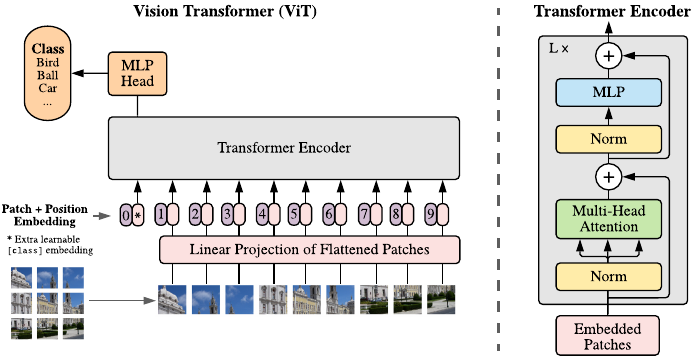
\includegraphics[width=\textwidth]{pictures/vit}\\
    \caption[Vision Transformer model structure]{Model overview. An image is split into fixed-size patches, each of them is linearly embedded, the position embeddings are added, and the resulting sequence of vectors feed to a standard Transformer encoder. In order to perform classification, the standard approach of adding an extra learnable “classification token” to the sequence is used. Figure and caption from~\autocite{Dosovitskiy2021}}
    \label{fig:vit}
\end{figure}

When the task is image classification an additional embedding is added, which will code as class token, once the training ended, according to~\autocite{Devlin2019}.
This embedded input will be fed into a standard Transformer encoder.~\autocite{Dosovitskiy2021}
The result of the encoder stack is a feature vector consisting of results for all the input embeddings.
For classification only the classification token is considered, all other features are ignored in this context, but they do represent features of the image and can be used for example for image segmentation, as explained shortly.

\begin{figure}[!t]
    \centering
    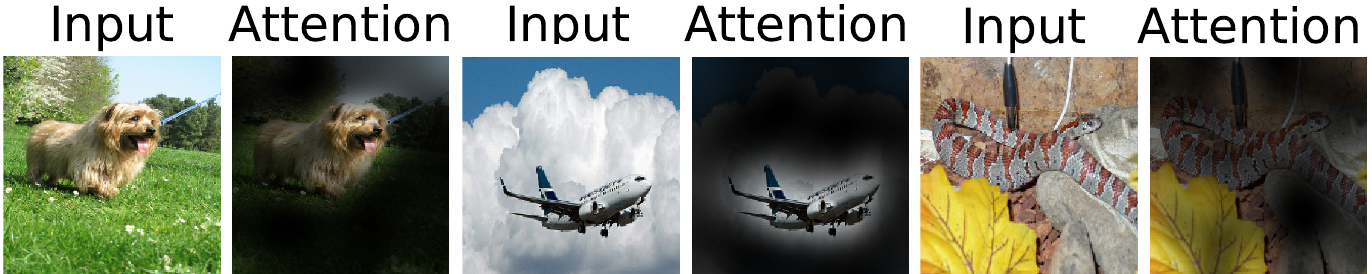
\includegraphics[width=\textwidth]{pictures/vit-attention2}\\
    \caption[Examples of attention in Vision Transformers]{Representative examples of attention from the output token to the input space of a Vision Transformer. Figure and caption from~\autocite{Dosovitskiy2021}}
    \label{fig:vit-attention}
\end{figure}

% what ViTs can do:
The self-attention mechanism allows the Vision Transformer to integrate information from across the whole image in all layers,meaning that the receptive field is broad~\autocite{Dosovitskiy2021}.
This is in contrast to Convolutional Neural Networks, which do tend to have more narrow receptive fields, due to how the convolution algorithm works.
Additionally, Transformers are still able to have smaller attention distances in the low layer, meaning they can still resolve local features.
Overall it was found, that the model attends to image regions that are semantically relevant~\autocite{Dosovitskiy2021}, as seen in~\autoref{fig:vit-attention}.
As mentioned before, for image classification only the classification token is considered, all other features are dropped.
%Transition to unsupervised segmentation
However, as it can be seen in the attention maps, these features contain semantic information about the image, and thus can be used for semantic segmentation.
Thus, shortly after the Vision Transformer was introduced for image classification~\autocite{Dosovitskiy2021}, algorithms were introduced that utilise these features for image segmentation tasks, for example by adding a projection head, that clusters the features~\autocite{Caron2021}.
It was even found, that features learned in an unsupervised fashion do contain even more relevant information, which can be used for clustering to generate a segmentation map of the input image~\autocite{Caron2021}.

 \subsubsection{Unsupervised Vision Transformer DINO}
% DINO - interpreting feature/attention maps, but make it self-supervised
Features learned in an unsupervised way provide a richer signal, since limiting the training to predefined concepts (for example to classification categories), reduces the rich visual information an image contains~\autocite{Caron2021}.
With unsupervised learning, information of an image assigned to another category might be utilised to build meaningful representations of that category or even completely unnamed (but nevertheless meaningful categories or semantic concepts).%\footnote{For example, learning representations of sky, even though that was not the intention of detecting street signs, might be helpful in figuring out the scene}.

The most successful unsupervised segmentation algorithm to date is called \gls{dino}\footnote{Knowledge distillation is a learning paradigm, where a student network is trained to match a teacher network~\autocite{Caron2021}.} uses a pair of Vision Transformers as student and teacher networks (($g_{\theta_s}$) and $g_{\theta_t}$)\footnote{Other networks can be used as backbone, but Vision Transformers were found to perform exceptionally well~\autocite{Caron2021}.}.

The forward pass in each network is calculated as following (example given for student network):
\begin{equation}
    P_s(x)^{(i)} = \frac{exp(g_{\theta_s}(x)^{(i)} / \tau_s)}{exp(\sum^K_{k=1}g_{\theta_s}(x)^{(k)} / \tau_s)}
    \label{eq:forward-pass}
\end{equation}
Where $\tau_s > 0$ is a temperature parameter to control sharpness of the output distribution.
Since student and teacher architecture are the same, output of the teacher will be calculated analogously.

\begin{figure}[!t]
    \centering
    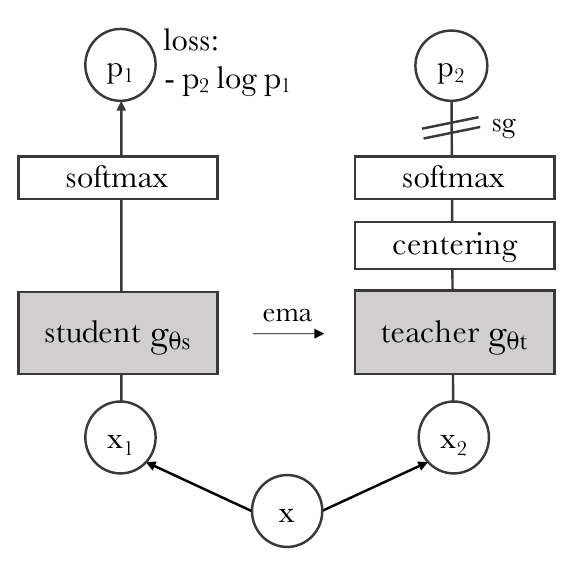
\includegraphics[width=0.6\textwidth]{pictures/dino-structure}\\
    \caption[Structure of DINO]{Self-distillation with no labels. Illustration of DINO in the case of one single pair of views ($x_1$ , $x_2$ ) for simplicity. The model passes two different random transformations of an input image to the student and teacher networks. Both networks have the same architecture but different parameters. The output of the teacher network is centered with a mean computed over the batch. Each networks outputs a K dimensional feature that is normalized with a temperature softmax over the feature dimension. Their similarity is then measured with a cross-entropy loss. We apply a stop-gradient (sg) operator on the teacher to propagate gradients only through the student. The teacher parameters are updated with an exponential moving average (ema) of the student parameters. Figure and caption from~\autocite{Caron2021}}
    \label{fig:dino-structure}
\end{figure}

%backwardspass
The loss function of the student network is the cross entropy loss between teacher and student, while the weight update for the teacher is done by an exponential moving average (also known as momentum encoder) from the students weights~\autocite{Caron2021}.

For training, each network gets different crops of the same image (taken from a set of views $V$ of the image), but only global crops $x^g_i$(comprising more than half the input image area) are passed to the teacher, while the student gets local and global crops, to encourages a local-to-global correspondence~\autocite{Caron2021}.
Thus, the loss function in the student to be minimised is:
\begin{equation}
    \min_{\theta_s} \sum_{x \in \{x^g_1, x^g_2\}} \sum_{\substack{x' \in V \\ x' \neq x}} H(P_t(x), P_s(x'))
    \label{eq:loss-with-crops}
\end{equation}
Where $H$ is the cross entropy loss $H(a,b) = -a log(b)$.

As mentioned earlier, the weight update in the teacher will be done by an exponential moving average from the students weights.
Additionally, to avoid collapse in the teacher network centering and sharpening is used on the output before applying the softmax function.\footnote{There were found two forms of collapse: regardless of the input, the model output is uniform along all the dimensions or dominated by one dimension.}
Centering was found to hinder one dimension to dominate, but may encourage collapse to a uniform distribution.
Sharpening has an opposite effect.
So, combining both was found to stabilise the model.~\autocite{Caron2021}

\begin{figure}[!t]
    \centering
    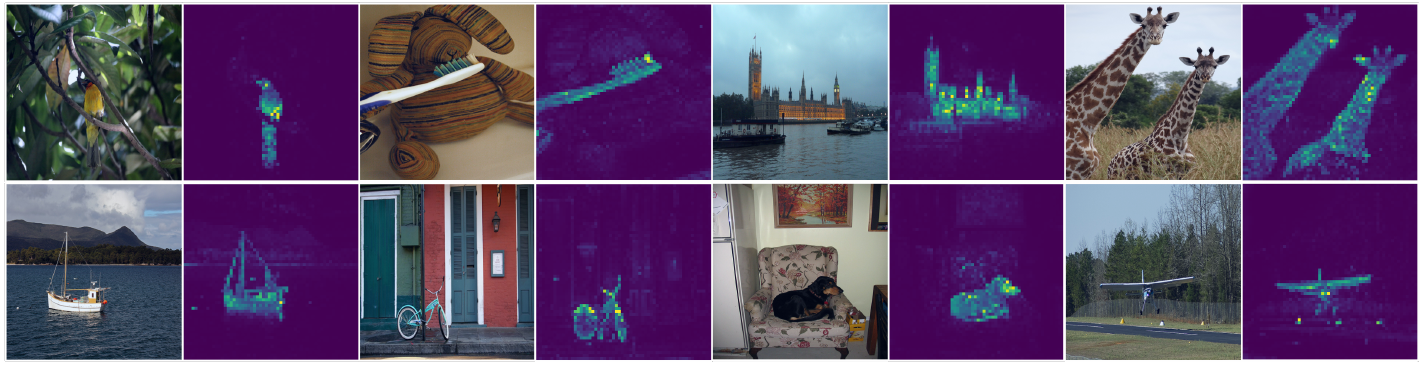
\includegraphics[width=\textwidth]{pictures/dino-attentionmaps}\\
    \caption[Self-attention maps of DINO]{Self-attention from a Vision Transformer with 8 × 8 patches trained with no supervision. We look at the self-attention of the classification token on the heads of the last layer. This token is not attached to any label nor supervision. These maps show that the model automatically learns class-specific features leading to unsupervised object segmentations. Figure and caption from~\autocite{Caron2021}}
    \label{fig:dino-attentionmaps}
\end{figure}

% results of DINO
When evaluating this set-up, the authors found that different segmentation heads are even found to attend to different semantic regions of an image even when they are occluded, meaning they are specialised to detect certain semantic patterns~\autocite{Caron2021}.
Additionally, the self-attention maps associated with a classification token (the name of this now unsupervised token was maintained for consistency with previous works) show that the architecture automatically learned class-specific features, as seen in~\autoref{fig:dino-attentionmaps}.
Even though neither the training objective nor the architecture where designed for such dense tasks, the self-attention maps could be used straight away as segmentation maps, yielding up to 71.4~\% region similarity and contour accuracy~\autocite{Caron2021}.

This underlines the huge potential the self-attention maps of an unsupervised Vision Transformer have, and not long after \gls{dino} was published, an architecture followed which expanded \gls{dino} by adding an energy based graph optimisation to better generate segmentation masks from the self-attention maps~\autocite{Hamilton2022}.
This architecture is called \glsfirst{stego}.





